%\documentclass[handout]{ximera}
\documentclass{ximera}

\usepackage{gensymb}
\usepackage{tabularx}
\usepackage{mdframed}
\usepackage{pdfpages}
%\usepackage{chngcntr}

\let\problem\relax
\let\endproblem\relax

\newcommand{\property}[2]{#1#2}




\newtheoremstyle{SlantTheorem}{\topsep}{\fill}%%% space between body and thm
 {\slshape}                      %%% Thm body font
 {}                              %%% Indent amount (empty = no indent)
 {\bfseries\sffamily}            %%% Thm head font
 {}                              %%% Punctuation after thm head
 {3ex}                           %%% Space after thm head
 {\thmname{#1}\thmnumber{ #2}\thmnote{ \bfseries(#3)}} %%% Thm head spec
\theoremstyle{SlantTheorem}
\newtheorem{problem}{Problem}[]

%\counterwithin*{problem}{section}



%%%%%%%%%%%%%%%%%%%%%%%%%%%%Jenny's code%%%%%%%%%%%%%%%%%%%%

%%% Solution environment
%\newenvironment{solution}{
%\ifhandout\setbox0\vbox\bgroup\else
%\begin{trivlist}\item[\hskip \labelsep\small\itshape\bfseries Solution\hspace{2ex}]
%\par\noindent\upshape\small
%\fi}
%{\ifhandout\egroup\else
%\end{trivlist}
%\fi}
%
%
%%% instructorIntro environment
%\ifhandout
%\newenvironment{instructorIntro}[1][false]%
%{%
%\def\givenatend{\boolean{#1}}\ifthenelse{\boolean{#1}}{\begin{trivlist}\item}{\setbox0\vbox\bgroup}{}
%}
%{%
%\ifthenelse{\givenatend}{\end{trivlist}}{\egroup}{}
%}
%\else
%\newenvironment{instructorIntro}[1][false]%
%{%
%  \ifthenelse{\boolean{#1}}{\begin{trivlist}\item[\hskip \labelsep\bfseries Instructor Notes:\hspace{2ex}]}
%{\begin{trivlist}\item[\hskip \labelsep\bfseries Instructor Notes:\hspace{2ex}]}
%{}
%}
%% %% line at the bottom} 
%{\end{trivlist}\par\addvspace{.5ex}\nobreak\noindent\hung} 
%\fi
%
%


\let\instructorNotes\relax
\let\endinstructorNotes\relax
%%% instructorNotes environment
\ifhandout
\newenvironment{instructorNotes}[1][false]%
{%
\def\givenatend{\boolean{#1}}\ifthenelse{\boolean{#1}}{\begin{trivlist}\item}{\setbox0\vbox\bgroup}{}
}
{%
\ifthenelse{\givenatend}{\end{trivlist}}{\egroup}{}
}
\else
\newenvironment{instructorNotes}[1][false]%
{%
  \ifthenelse{\boolean{#1}}{\begin{trivlist}\item[\hskip \labelsep\bfseries {\Large Instructor Notes: \\} \hspace{\textwidth} ]}
{\begin{trivlist}\item[\hskip \labelsep\bfseries {\Large Instructor Notes: \\} \hspace{\textwidth} ]}
{}
}
{\end{trivlist}}
\fi


%% Suggested Timing
\newcommand{\timing}[1]{{\bf Suggested Timing: \hspace{2ex}} #1}




\hypersetup{
    colorlinks=true,       % false: boxed links; true: colored links
    linkcolor=blue,          % color of internal links (change box color with linkbordercolor)
    citecolor=green,        % color of links to bibliography
    filecolor=magenta,      % color of file links
    urlcolor=cyan           % color of external links
}

\title{Congruence Criteria}
\author{Bart Snapp and Brad Findell}

\outcome{Learning outcome goes here.}

\begin{document}
\begin{abstract}
Abstract goes here.  
\end{abstract}
\maketitle

\begin{teachingnote}
Perhaps ask students to come up with the sequence of transformations. 

Discuss a common error:   Translate $\triangle ABC$ through the vector $\overrightarrow{BY}$.  Then rotate about $Y$ by $\angle C'YZ.$. 

The generality of the proofs requires consideration of the possibility that a reflection might not be necessary in the general case.  Use half-plane ideas to ask whether points are on the same side or opposite sides of lines.  

Simplify by eliminating the prime notation.  After the translation, for example, $A$ coincides with $X$.  (See photos from class.)
\end{teachingnote}

In this activity, we show how the common triangle congruence criteria follow from
 what we now know about isometries.%\standardhs{G-CO.8}  
 Recall that two figures are said to be 
congruent if there exists an isometry (translation, rotation, or reflection) or a 
sequence of isometries that maps one figure onto the other.  
\fixnote{Cite CCSS G-CO.8.}

\begin{problem}
Proof of Side-Angle-Side (SAS) congruence.  Suppose $\triangle ABC$ and $\triangle XYZ$ are such that $AB=XY$, $AC=XZ$, and $\angle A \cong \angle X$.  Prove, using basic rigid motions, that $\triangle ABC \cong \triangle XYZ$.  Consider the figure below.  
\begin{image}
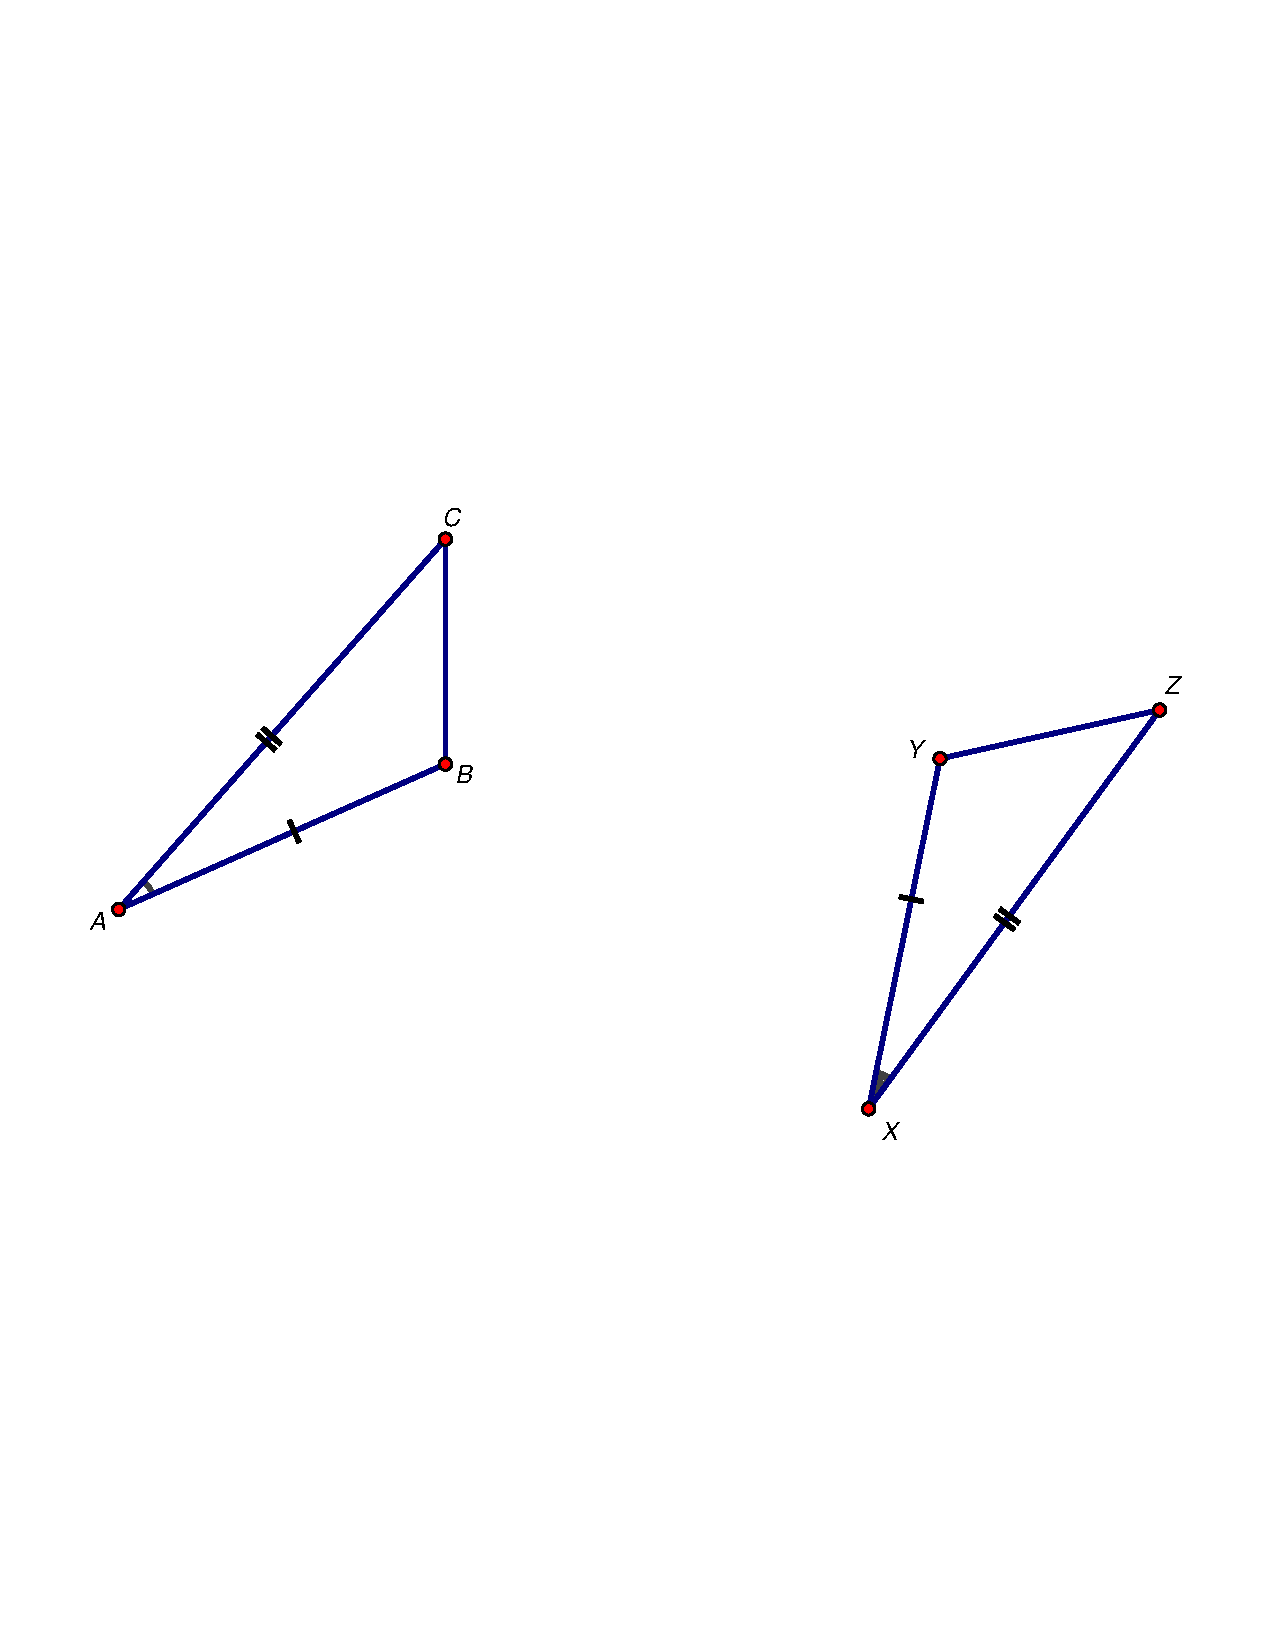
\includegraphics[scale=0.6]{SAS.pdf}
\end{image}
Fill in the details of the following proof.  
\begin{enumerate}
\item Translate $\triangle ABC$ through the vector $\overrightarrow{AX}$.  Call the image $\triangle A'B'C'$.  Explain why $A'$ and $X$ coincide.
\item Rotate $\triangle A'B'C'$ about $X=A'$ through $\angle B'XY$ so that ray $\overrightarrow{A'B'}$ is along ray $\overrightarrow{XY}$.  Call the image $\triangle A''B''C''$   Explain how you know the segments $\overline{A''B''}$ and $\overline{XY}$ coincide. 
\item Reflect $\triangle A''B''C''$ about the line $\overleftrightarrow{A''B''} = \overleftrightarrow{XY}$.  Call the image $\triangle A'''B'''C'''$.  Explain why $\overline{A'''C'''}$ and $\overline{XZ}$ coincide.
\item Explain how you now know that all sides and angles of $\triangle A'''B'''C'''$ are congruent to the corresponding sides and angles of $\triangle XYZ$.  
\item Explain how to modify the above steps to handle the following different cases: 
\begin{itemize}
\item Initially $X = A$. 
\item After the translation, $\overline{A'B'}$ and $\overline{XY}$ coincide. 
\item After the rotation, $\overline{A''C''}$ and $\overline{XZ}$ coincide.  (Hint:  Consider whether $C''$ and $Z$ are on the same side or on opposite sides of $\overleftrightarrow{XZ}$.)  
\end{itemize}
\end{enumerate}
\end{problem}

\begin{problem}
Proof of Angle-Side-Angle (ASA) congruence.  Suppose $\triangle ABC$ and $\triangle XYZ$ are such that $AB=XY$, $\angle A \cong \angle X$, and $\angle B \cong \angle Y$.  Prove, using basic rigid motions, that $\triangle ABC \cong \triangle XYZ$.  
\begin{enumerate}
\item Outline a general proof for the figure below.  
\begin{image}
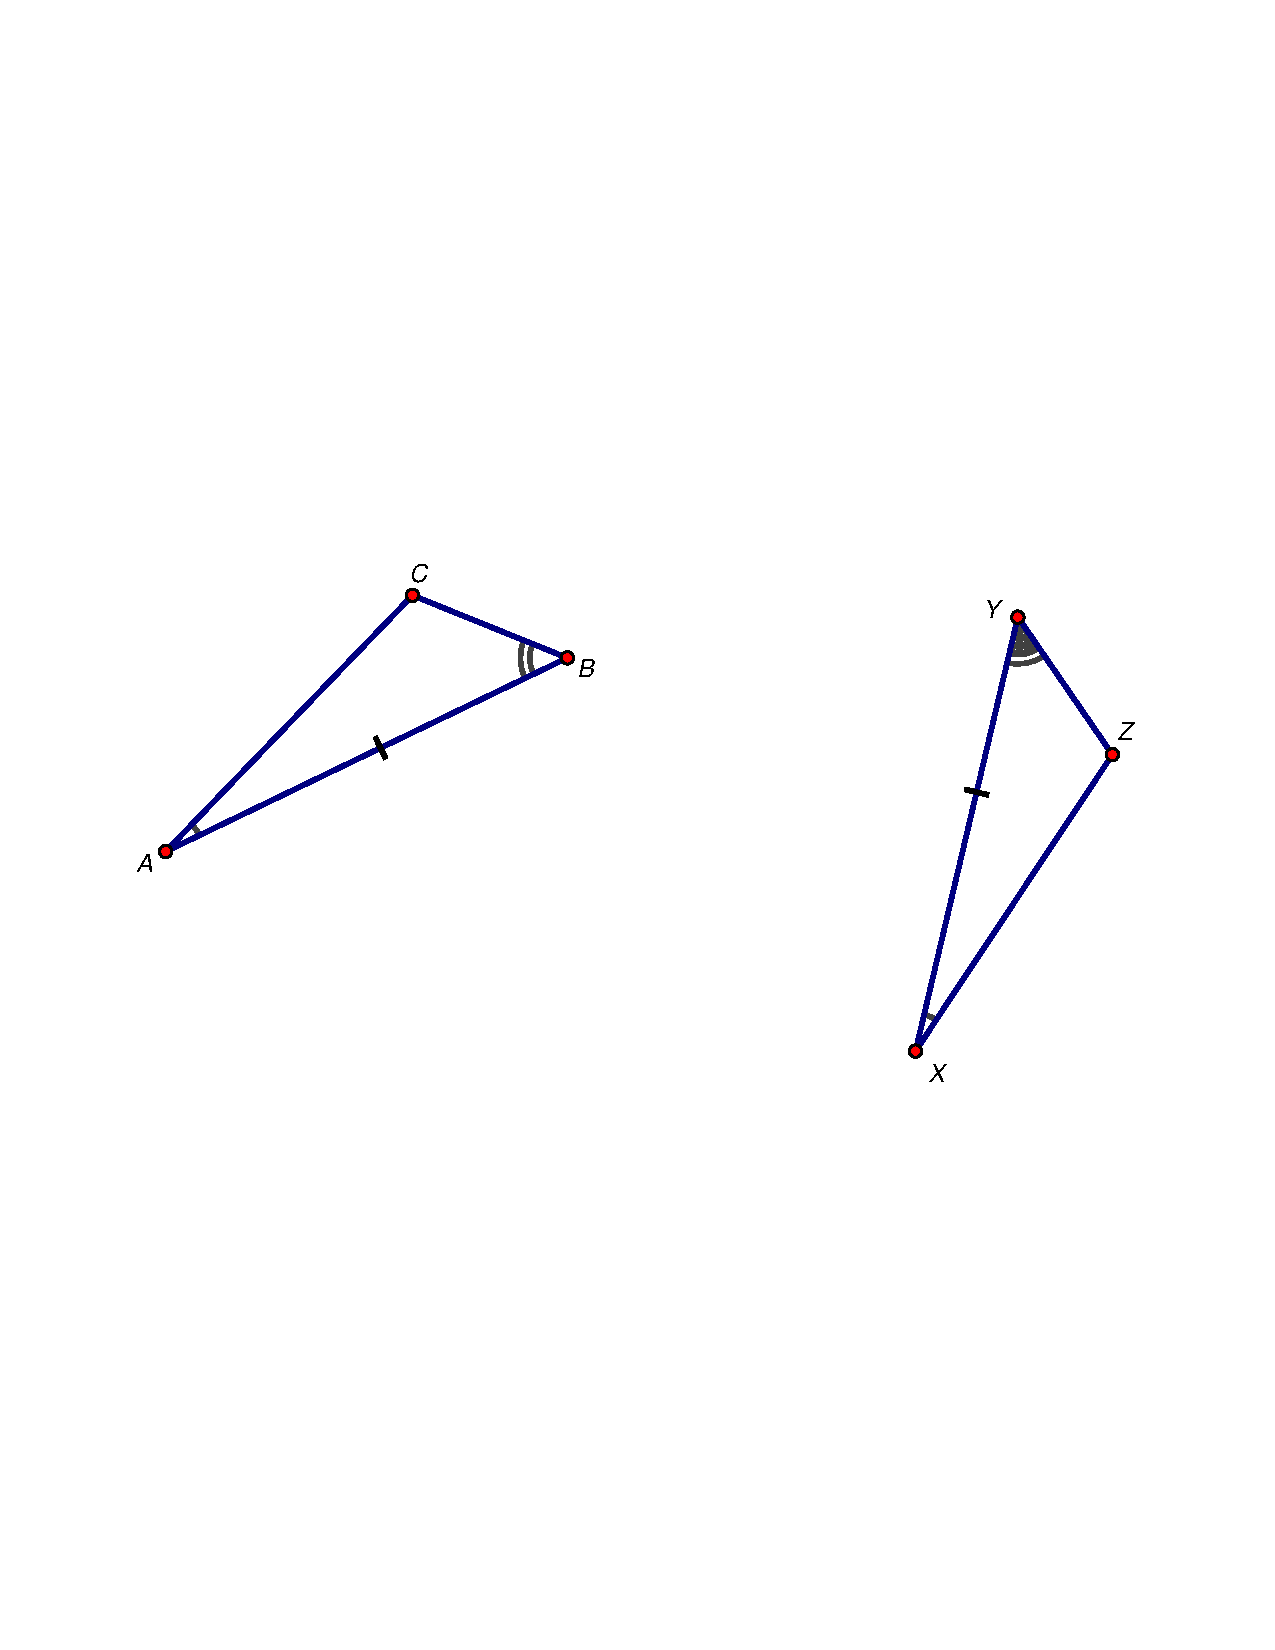
\includegraphics[scale=0.6]{ASA.pdf}
\end{image}
\item Explain carefully how you know, after the sequence of rigid motions, that the ``final image'' of $C$ coincides with $Z$.  
\item Describe how to modify the outline to handle other cases. 
\end{enumerate}
\end{problem}

\begin{problem}
In a previous activity, you used triangle congruence criteria to prove the following results: 
\begin{itemize}
\item The Isosceles Triangle Theorem.
\item The points on a perpendicular bisector of a segment are exactly those that are equidistant from the endpoints.
\end{itemize}
Verify that these results could have been established using only SAS and ASA congruence.  (Thus, you may use these results in the problems that follow.) 
\end{problem}

\begin{problem}
Proof of Hypotenuse-Leg (HL) congruence.  Suppose $\triangle ABC$ and $\triangle XYZ$ are such that $\angle C$ and $\angle Z$ are right angles, $AB=XY$, and $BC=YZ$.  Prove that $\triangle ABC \cong \triangle XYZ$.  
\begin{image}
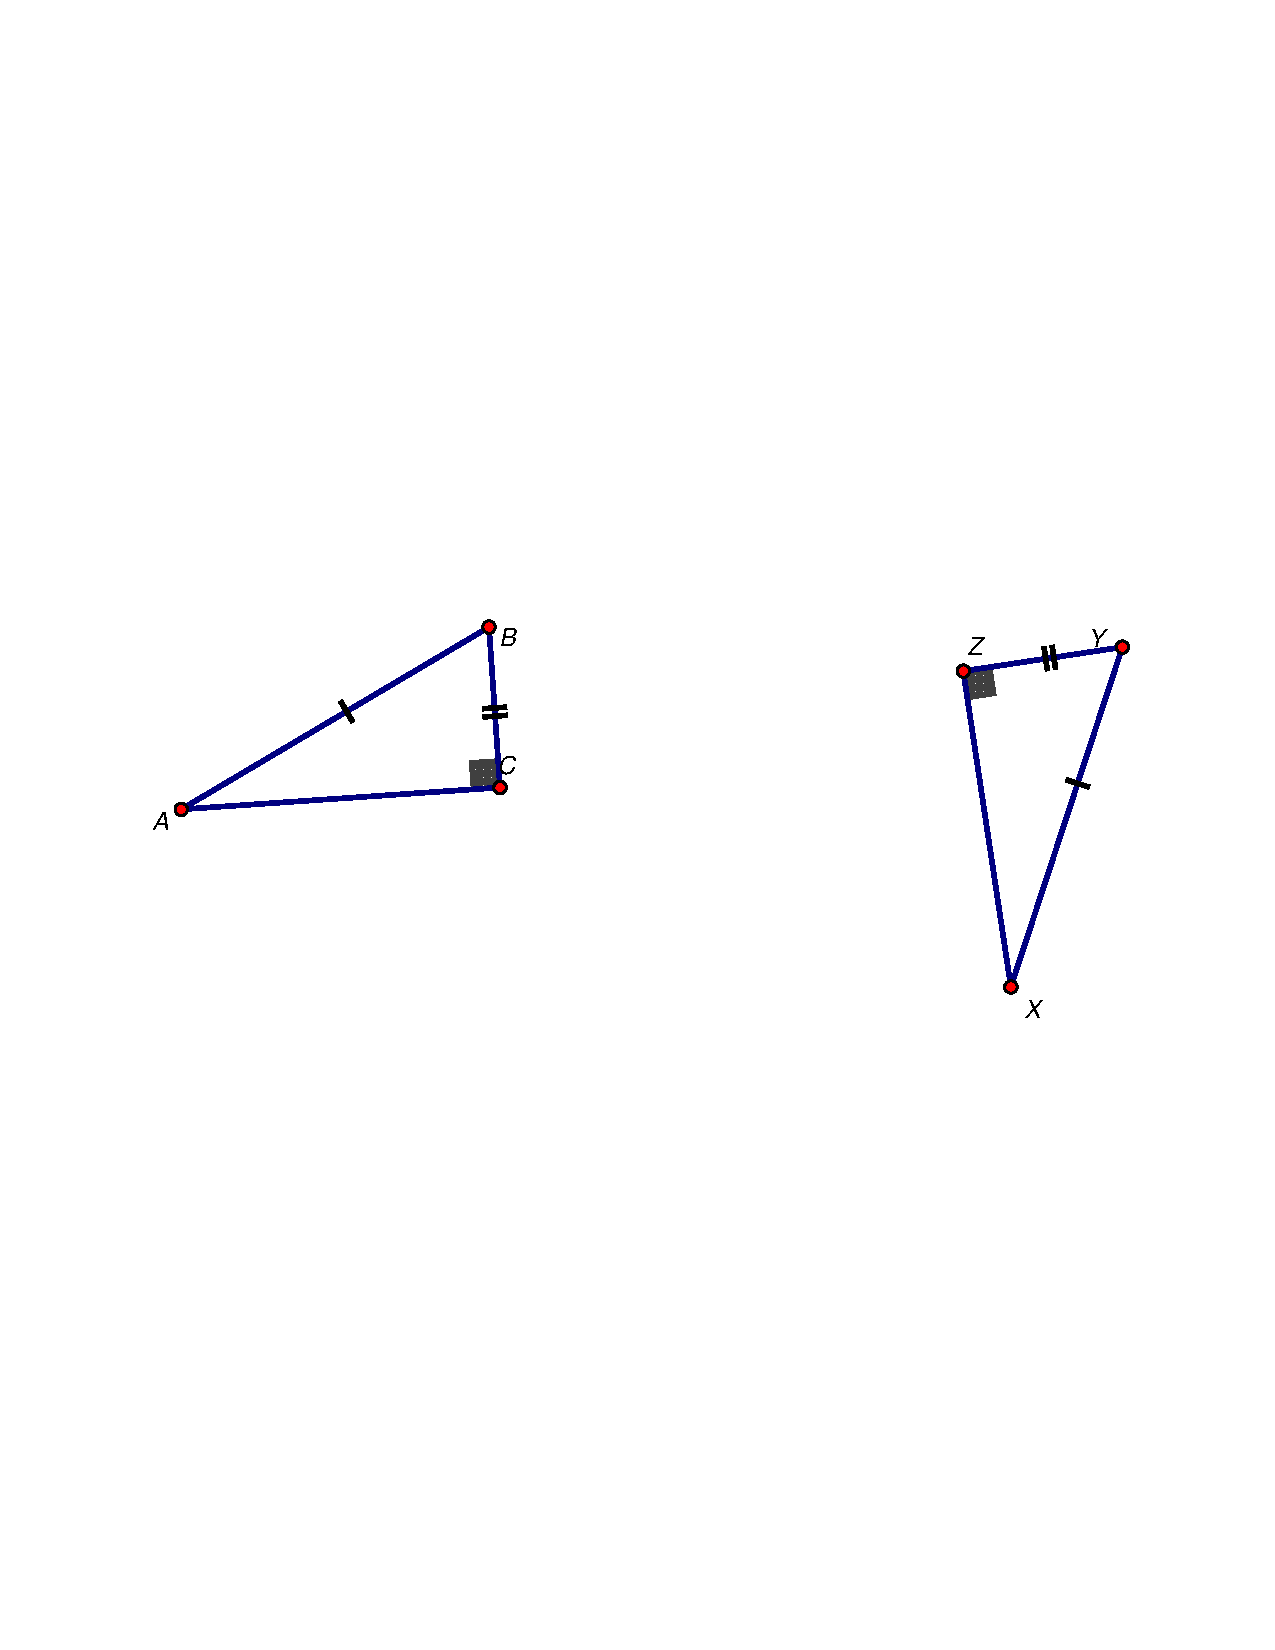
\includegraphics[scale=0.6]{HL.pdf}
\end{image}
\end{problem}

\begin{teachingnote}
One approach:  First extend side $\overrightarrow{AC}$ to a point $A'$ so that $CA'=XZ$, and argue that $\triangle A'BC \cong \triangle XYZ$.

Easier:  Translate $\triangle ABC$ through the vector $\overrightarrow{CZ}$.  Then rotate.

Alternatively, save HL until after SSS?
\end{teachingnote}


\begin{problem}
Proof of Side-Side-Side (SSS) congruence.  Suppose $\triangle ABC$ and $\triangle XYZ$ are such that $AB=XY$, $AC=XZ$, and $BC=YZ$.  Prove, using basic rigid motions, that $\triangle ABC \cong \triangle XYZ$.  Build toward the general case through the following steps:  
\begin{teachingnote}
Or maybe these two figures don't matter if we emphasize that $A$ and $B$ both lie on the perpendicular bisector of $\overline{CZ}$.
\end{teachingnote}
\begin{enumerate}
\item Case 1a:  $A=X$, $B=Y$, and $C$ and $Z$ lie on opposite sides of $\overleftrightarrow{AB}$.  (Hint:  Explain why the situation must be like one of the figures below, argue that $\overleftrightarrow{AB}$ is the perpendicular bisector of $\overline{CZ}$, and then use a reflection.)
\begin{image}
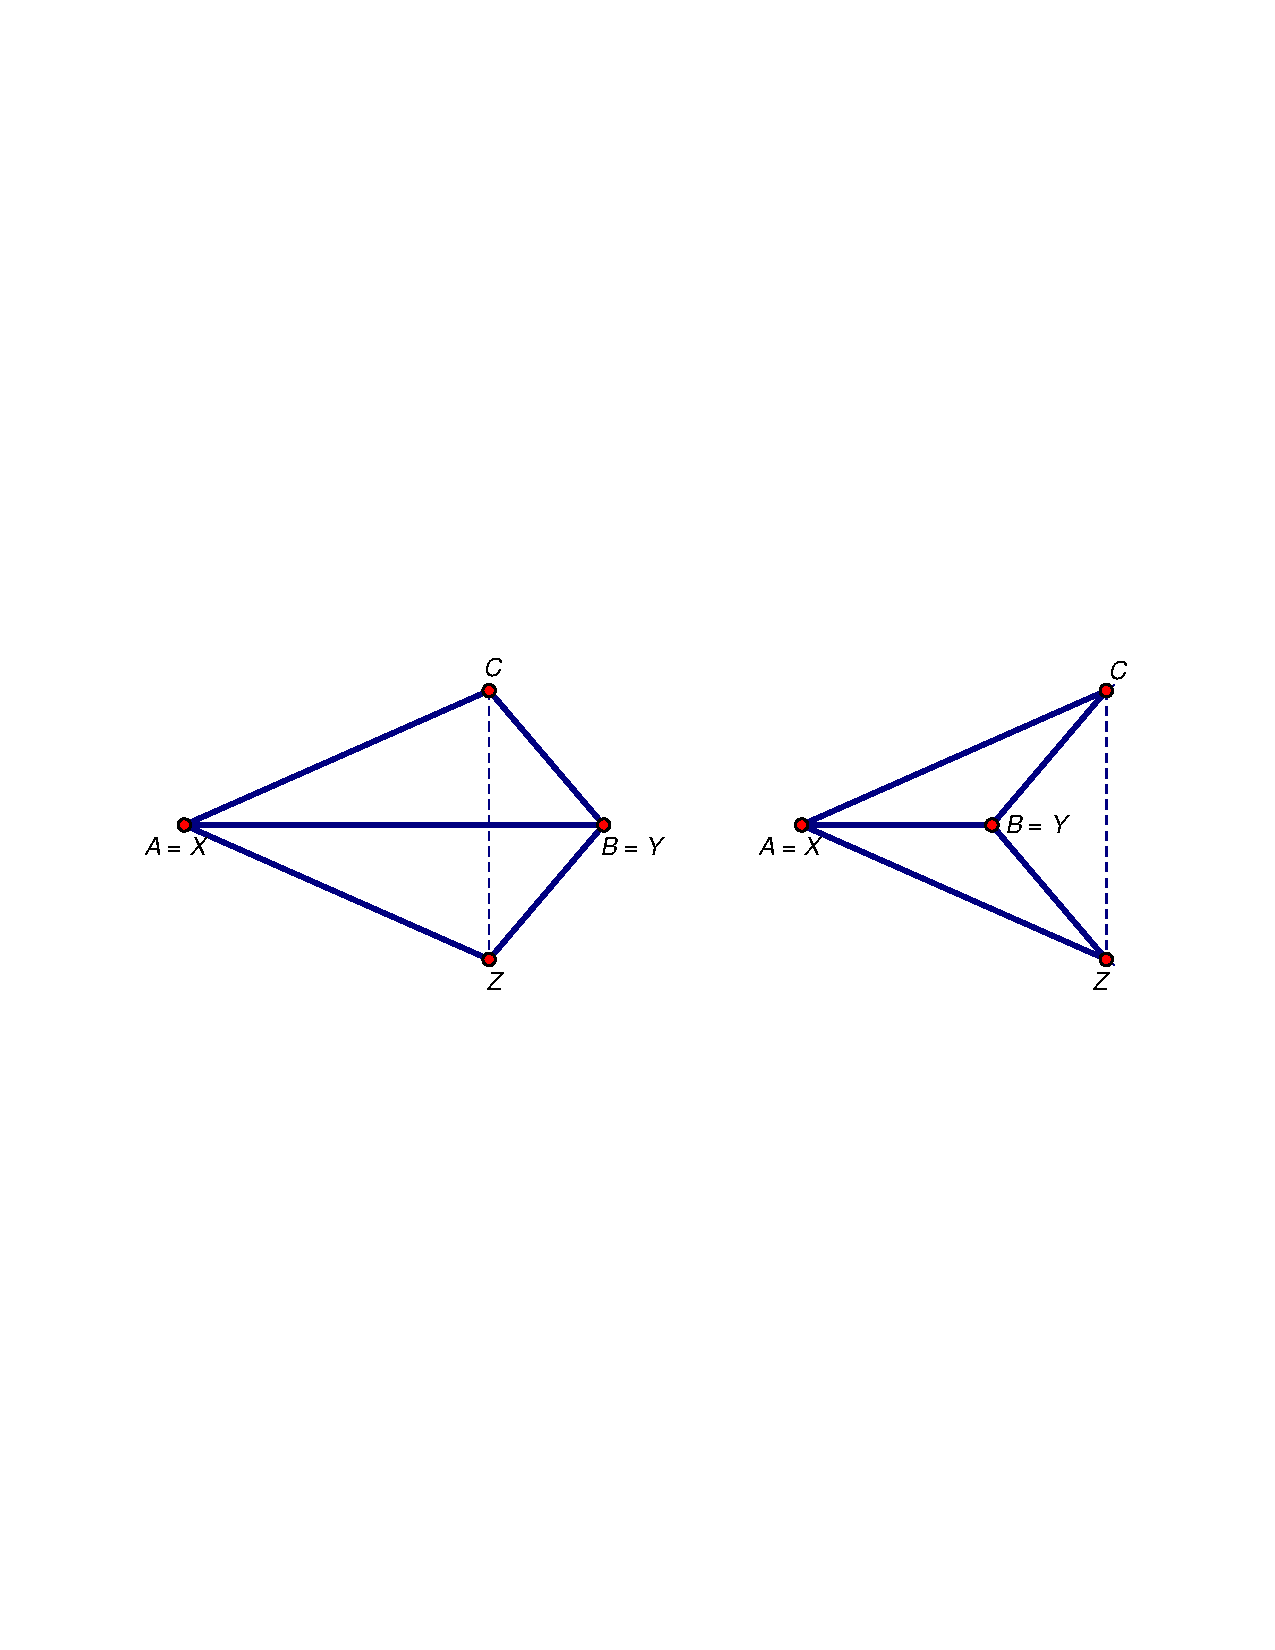
\includegraphics[scale=0.6]{SSS.pdf}
\end{image}
\item Case 1b:  $A=X$, $B=Y$, and $C$ and $Z$ lie on the same side of $\overleftrightarrow{AB}=\overleftrightarrow{XY}$.  (Hint: Consider a reflection of one of the triangles and use the previous case.)  
\item Case 2:  $A=X$ but $B \ne Y$.
\item Case 3: The general case.  
\end{enumerate}
\end{problem}

\end{document}
